\chapter{Related Work} \label{chap:relat}
This chapter is the start of our research and describes our literature study of ubicomp, AR and feedforward. We provide context by discussing both history and current work. Our focus, however, is on interaction techniques combining two or all of the aforementioned concepts, since we will be designing such interaction techniques ourselves in the next chapter, as part of our exploration of the design space.

\section{History of AR} \label{sec:relat:ar}
A minimal VR prototype is technologically simpler than a minimal AR prototype, since VR requires ``only'' a (stereoscopic) display, a way to track the user's orientation, and a rendering engine to create the virtual world. AR requires these same capabilities, plus an internal model of the environment and a way to overlay images on a view of the real world, like a live camera feed or a semi-transparent display. Additionally, AR is more sensitive to processing delays and inaccurate sensors, since these can cause offsets between the world view and the virtual overlay. In VR, such offsets do not exist, so tracking delays and errors are generally less noticeable. It is not surprising then that VR is the historic predecessor to AR, and that because of their similarities, development of the two technologies has often been intertwined.

Ivan Sutherland, named by many as the father of computer graphics, published his vision of the Ultimate Display in 1965 \cite{sutherland1965ultimate}. He pointed out that conventional computers use a screen that only partially occupies user's vision, sometimes complemented with sound, and that other senses typically are left untouched. Input is registered via keyboard, joystick, or a similar device. Sutherland argued that these approaches severely limit our interaction methods, and therefore the ways in which computers can be used. The ultimate display would be a system that takes full control over all of the user's senses, and that could register every slight movement of the user's body. It could then create any conceivable experience for the user and adapt to their every motion. Experiences in this display would not even be limited by the laws of physics, since the display could simulate concepts like negative gravity or materials not found in the real world. What Sutherland envisioned, we might now call the ultimate VR system, or the ultimate AR system when complemented with knowledge of the real world.

The Sword of Damocles \cite{sutherland1968head}, shown in Figure \ref{fig:sword_of_damocles}, was developed mainly by Ivan Sutherland in 1968 and is widely considered to be the first functional VR setup. The system used a heavy HMD (head-mounted display) that had to remain attached to bars above the user's head, which is also where the name comes from. The system could track the user's head rotation, allowing them to look around in the virtual world, and even allowed for some small movement. Limited processing power meant the virtual world consisted of simple wireframe figures, however these were sufficient to prove the system functional.

\begin{figure}
    \centering
    \includegraphics[width=1.0\linewidth]{resources/introduction/sword_of_damocles.jpg}
    \caption{The Sword of Damocles (1968) \cite{sutherland1968head}.}
    \label{fig:sword_of_damocles}
\end{figure}

The first true AR system was introduced nearly 25 years after the Sword of Damocles. In 1992, Louis Rosenberg developed virtual fixtures for the U.S. Air Force \cite{rosenberg1992use}. The system was designed for assisting in remotely manipulated tasks, like operating a robotic arm or driving a remote-controlled vehicle, possibly without direct line of sight with the device in question. To use the system, the user wears a HUD and a full upper-body exoskeleton. The HUD provides a live camera feed of the task being performed, and the user's arm movements are relayed to the device for control. In case of the robotic arm, the camera position and orientation continually line up so that the robotic arm appears in place of the user's real arm. The robotic arm then mimics the user's arm movements, letting the user work like the task were performed in person rather than remotely.

To assist in task execution, Rosenberg's system introduces virtual fixtures, which are sensory overlays that guide the user towards the desired actions. Specifically, the exoskeleton can resist the user's actions with varying degrees of force, nudging them towards the desired movements. We distinguish \textit{guiding virtual fixtures}, which exert limited force that can be overcome by the user, and \textit{forbidden regions virtual fixtures}, which prevent the user from making some movements. The latter can simulate an invisible wall that a robotic arm cannot move through or a remote-controlled vehicle cannot not drive past, and can for example be used for safety restrictions. However, virtual fixtures as proposed by Rosenberg are not limited to guiding the user's movements, and neither do they have to be haptic. Their general goal is to improve user awareness and localization. This can also be achieved via visual cues, like rendering the haptic ``force fields'' in the user's view, and via auditory cues, like a buzzing sound that becomes more urgent the more the user deviates from the ideal path. Rosenberg's study showed that a simple combination of haptic and auditory virtual fixtures increase user performance by up to 70\% in remote tasks, like using a robotic arm to place pegs in specific holes.

\begin{figure}
    \centering
    \includegraphics[width=0.8\linewidth]{resources/introduction/virtual_fixtures.jpg}
    \caption{Virtual Fixtures (1992) \cite{sutherland1968head}.}
    \label{fig:virtual_fixtures}
\end{figure}

The rest of the 90s and the 00s brought a large variety of AR applications, and not all of them used HMD's. The aviation and automotive industries developed HUD's (head-up display) projecting navigational aids and system information over the windshield. Several companies developed apps that can translate text on the fly when viewed through a smartphone. In 2013, Google released their Google Glass, which is voice-controlled and can display information in the user's peripheral vision. In 2016, Microsoft brought their HoloLens to market, a HMD with spatial awareness and a transparent display that it uses to place virtual interactive objects, which they call \textit{holograms}, in the real world. Since then, the number of AR devices has started to grow more quickly, but as mentioned in Chapter \ref{chap:intro}, they are still mostly targeted at professionals.

\begin{figure}
    \centering
    \includegraphics[width=0.8\linewidth]{resources/introduction/hololens.jpg}
    \caption{Microsoft HoloLens (2016).}
    \label{fig:hololens}
\end{figure}

\section{Feedforward} \label{sec:relat:feedforward}
Feedforward, as mentioned in Chapter \ref{chap:intro}, is the process of telling the user what is going to happen if they proceed with an action. This is different from Norman's \textit{affordances} \cite{norman2013design}, which show only the potential for an action, without conveying its possible effects \cite{chueke2016perceptible}.

\citeauthor{djajadiningrat2002but} (\citeyear{djajadiningrat2002but}) argue that ``both appearance and action are carriers of meaning'' \cite{djajadiningrat2002but}, or in other words, a UI element can express its purpose both via its appearence and via its available actions.

\todo{Discuss the different views on feedforward, as given by

\citeauthor{djajadiningrat2002but} \cite{djajadiningrat2002but}, \citeauthor{wensveen2004interaction} \cite{wensveen2004interaction}
\citeauthor{vermeulen2013crossing} \cite{vermeulen2013crossing}.

A good comparison has previously been made by \citeauthor{chueke2016perceptible} \cite{chueke2016perceptible}. Also missing \cite{djajadiningrat2004tangible}.}

\section{Gesture-based Commands} \label{sec:relat:gesture-based_commands}
In ubicomp environments, the user should be able to interact with the system in a way that feels natural, and preferably they are able to move around freely while doing so. Gesture-based commands allow the user to describe their intention with motions, which may be more convenient than pressing buttons in some cases, and mid-air gestures do not lock the user in place. We will now discuss some earlier works on gesture-based commands and their possible advantages.

\textbf{OctoPocus} explores the use of feedforward in on-screen gesture-based commands \cite{bau2008octopocus}. When the user initiates a command, for each possible gesture a labeled path radiates from the cursor, giving the user feedforward by telling them what will happen if they move the cursor in a particular way (Fig. \ref{fig:bau2008octopocus_demo}). The accompanying user study indicates that this approach allows for lower overhead in time than when using traditional help menus, that it is less error-prone, allows for ``in situ'' learning, and that it is generally preferred by users.

\begin{figure}
    \centering
    \includegraphics[width=0.7\linewidth]{bau2008octopocus/example.png}
    \caption{Example of \textbf{OctoPocus} with three possible commands: tracing a gesture (\textit{copy} in this case) causes other gestures to get thinner (like \textit{cut}) and completely disappear when they become too distinct (like \textit{paste}) \cite{bau2008octopocus}}
    \label{fig:bau2008octopocus_demo}
\end{figure}

\textbf{Shadow Tooltips} are a feedforward concept for multi-touch devices \cite{freitag2012enhanced}. When a user's hand approaches the screen, labeled silhouettes of the hand appear around it, conveying the different possible actions the hand can take and their corresponding effect (Fig. \ref{fig:freitag2012enhanced_demo}). In the accompanying qualitative user study, Shadow Tooltips scored very high on \textit{novelty}, high on \textit{appeal}, \textit{ease of use} and \textit{comprehensibility}, and moderate on \textit{relevance}, meaning the users enjoyed trying out the concept, but were divided on its practicality.

\begin{figure}
    \centering
    \includegraphics[width=0.7\linewidth]{freitag2012enhanced/example.png}
    \caption{Example of \textbf{Shadow Tooltips} in which the left hand can drag the map with one finger and zoom with two fingers, while each of the right hand fingers can be used for drawing \cite{freitag2012enhanced}}
    \label{fig:freitag2012enhanced_demo}
\end{figure}

\todo{Add Gestu-Wan \cite{rovelo2015gestu}.}


\begin{figure}
    \centering
    \includegraphics[width=0.6\linewidth]{rovelo2015gestu/schema.jpg}
    \caption{Illustration of \textbf{Gestu-Wan}, with annotation by the authors: ``Step (1): (A) shows the previously matched posture, while (B) is the target posture. Step (2): When the target posture is matched, it moves up and the tree expands to show the next steps. Step (3): All the next possible postures are shown and the user can match one of them to continue with the gesture''. \cite{freitag2012enhanced}}
    \label{fig:rovelo2015gestu_schema}
\end{figure}

\section{AR Projectors} \label{sec:relat:ar_projectors}
\textbf{\citeauthor{vermeulen2009bet}} use a series of mounted projectors to visualize the different input/output devices present in a room \cite{vermeulen2009bet}. Close to the physical location of each device, they project an icon that resembles it, making all devices clearly visible to the user. The different possible events that input devices can detect are visualized by labels connected to the device's icon. From these events, lines are drawn to the actions that they trigger, and these actions in turn have lines running to the output devices on which they occur (Fig. \ref{fig:vermeulen2009bet_mockup}, \ref{fig:vermeulen2009bet_demo}). This setup gives the user extensive feedforward, since it tells them the exact results of every possible action they can take. The accompanying informal user study yielded promising results, with four of the five participants describing the system's behavior correctly for each of three presented tasks, and all participants indicating that they found the system useful. However, some shortcomings were identified too: it can be hard to keep track of visualizations across multiple surfaces, and visualizations for actions that are obvious or occur often can be confusing and might better be left out.

\begin{figure}
    \centering
    \includegraphics[width=0.7\linewidth]{vermeulen2009bet/example.png}
    \caption{Example of \textbf{\citeauthor{vermeulen2009bet}}'s concept in which a touchscreen can detect a \textit{click} event, which will cause a movie to start playing on the touchscreen and will cause the lights to dim \cite{vermeulen2009bet}}
    \label{fig:vermeulen2009bet_mockup}
\end{figure}

\begin{figure}
    \centering
    \includegraphics[width=0.7\linewidth]{vermeulen2009bet/demo.png}
    \caption{Demonstration of \textbf{\citeauthor{vermeulen2009bet}}'s concept showing how the user gets a clear view of which devices exist around them and how they are interconnected \cite{vermeulen2009bet}}
    \label{fig:vermeulen2009bet_demo}
\end{figure}

The \textbf{Feedforward Torch} is a hand-held mobile projector with a touchscreen, that can be aimed at legacy hardware interfaces to either project textual or graphical clarifications on them, or to show these clarifications on the on-board screen (Fig. \ref{fig:vermeulen2012understanding_demo}) \cite{vermeulen2012understanding}. In the accompanying small user study, all participants indicated they found the system useful. Visualizations were preferred over textual explanations and the participants appreciated the fact that information was overlaid on the associated interface rather than displayed on a mobile screen, which eliminated the need to look back and forth but also brings privacy concerns. The research team concludes that the concept could be valuable in helping users interact with systems that are complex or that suffer from design flaws.

\begin{figure}
    \centering
    \includegraphics[width=0.7\linewidth]{vermeulen2012understanding/demo.png}
    \caption{The user aims the \textbf{Feedforward Torch} at a set of unlabeled light switches to receive clarification \cite{vermeulen2012understanding}}
    \label{fig:vermeulen2012understanding_demo}
\end{figure}

\section{AR Note-taking} \label{sec:relat:ar_note-taking}
\todo{Add intro.}
\textbf{\citeauthor{liu2011mobile}} propose the use of mobile AR in note-taking \cite{liu2011mobile}. Looking through their PDA's, users can add annotations to the interfaces they aim at. These annotations later serve as feedforward when the users try to retrace their steps. The research team conducted no user study, but does mention challenges and opportunities, where the one concerning us in particular is how to convey rich annotations as clearly and efficiently as possible.

\begin{figure}
    \centering
    \includegraphics[width=0.7\linewidth]{liu2011mobile/demo.png}
    \caption{Demonstration of \textbf{\citeauthor{liu2011mobile}}'s concept in which the user looks through their PDA at an interface they've previously drawn virtual annotations on \cite{liu2011mobile}}
    \label{fig:liu2011mobile_demo}
\end{figure}

\section{Previewable Switch} \label{sec:relat:previewable_switch}
\todo{Add intro.}
The \textbf{Previewable Switch} presents feedforward as a solution to the spatial mapping problem of light switches \cite{park2014previewable}. When a switch is touched, the corresponding lights dim, giving the user feedforward on which lights will turn on or off if they continue their action (Fig. \ref{fig:park2014previewable_demo}). In the accompanied user study, participants consistently toggle lights faster and more accurately using these previewable switches than when using conventional switches, and they feel ``less work demand, reduced sensory time, and more comfort and confidence on their action''.

\begin{figure}
    \centering
    \includegraphics[width=0.7\linewidth]{park2014previewable/example.png}
    \caption{The user touches a \textbf{Previewable Switch}, which causes the corresponding light to dim \cite{park2014previewable}}
    \label{fig:park2014previewable_demo}
\end{figure}

%\section{Directional Indicators} \label{sec:related_work:directional_indicators}
%Talk about \cite{baudisch1993halo} and \cite{gustafson2008wedge}.

%\section{Scenarios} \label{section_scenarios}
%Many scenarios can be imagined where AR improves user experience by constituting feedforward. We divide these scenarios up into two categories, namely `setups in dumb environments' and `setups in smart environments', and for both of them, we discuss their advantages and give some examples.
%
%\subsection{Setups in Dumb Environments} \label{subsection_setups_in_dumb_environments}
%In these scenarios, the AR system cannot communicate with any other nearby systems. Often, this is because the nearby systems are simply not intelligent, but other reasons can also be thought of, like a lack of middleware required for communication. The AR system thus cannot change the environment and has to rely solely on its on-board sensors to gather information about its surroundings. To aid the system in this task, visual cues, e.g. QR codes, may be present.
%
%These setups are worth exploring because they are...
%\begin{itemize}
%    \item \textbf{low-cost}; the only material required is the AR system itself, plus potentially a set of visual cues, which come at any price, since they work just fine when printed in grayscale on plain paper.
%    \item \textbf{easy to set up}; no installation of peripherals is required, only the positioning of visual cues, if any.
%    \item \textbf{portable}; because setting up requires little to no work, moving to a different location is also easy. The setup can even exist simultaneously in different locations with little extra cost, since only the visual cues need to be duplicated, rather than having to buy and install multiple sets of peripherals.
%    \item \textbf{adaptable}; since setting up does not include careful installation of peripherals, changes are made more easily. What's more, if the AR system relies solely on visual cues for recognizing elements of interest, moving these cues suffices to relocate the elements, and adding more instances of an existing element is done by just creating more copies of its visual cue.
%    \item \textbf{noninvasive}; in some environments, like certain cultural heritage sites, drilling holes in the walls to hide peripherals and cables is unacceptable, and leaving them in plain sight spoils the view. Visual cues, on the other side, can be designed to blend in with the environment or, even better, can be comprised of objects already present.
%    \item \textbf{disposable}; in some contexts, people damaging or stealing peripherals can be a real concern. Especially in large outdoor or public areas, setting up expensive equipment may be deemed risky. Cheap, disposable visual cues can form a solution to this problem.
%\end{itemize}
%
%As a first example, let's consider a large museum, with several floors and many rooms. The museum currently provides audio guides, which are handheld devices that visitors carry with them for the duration of their stay. Every object of interest in the museum has a plaque with a unique number on it that visitors enter into their guides to hear a pre-recorded explanation about the object in question. This way, every visitor can finish the tour in any order they please, skip parts at will, hear explanations in their own language and replay them as often as they like. When this system works well, visitors have a great personalized experience.
%
%Let's assume there's no budget to install peripherals throughout the museum, because there are just way too many rooms. Even then, the museum is particularly well suited to be retrofitted for AR; procedures and infrastructure for handing out a personal device to every visitor are already present, and every object of interest already has a unique visual cue, mounted in a clearly visible location. Experiments must indicate if these existing number plaques can be recognized reliably by the AR systems, but even if they can't, another set of plaques can be installed when the old ones are due for replacement anyway, to save costs.
%
%In the museum, there are many ways in which AR can improve user experience, from highlighting relevant parts of objects during explanations, to small mini-games that can make the tour more engaging to children. However, we will not discuss these applications in more detail since our focus is specifically on feedforward.
%
%Imagine a visitor approaches an object of interest to take a closer look at it. The AR system detects this and displays a teacher icon in the user's peripheral vision to indicate that the associated explanation will shortly autoplay if the user does not interrupt. This is a perfect example of how AR can use feedforward to improve user experience, providing information about the near future without interrupting the user's current action.
%
%The visitor is now finished with the current room and wonders where to go to next. They look around and see three different exits, but can't remember where they've come from. In fact, they've just been wandering around the museum, pausing only at objects that caught their eye. This is where AR feedforward comes into play. Next to every door in the museum a unique painting is mounted, high enough as to always be visible and large enough to be recognizable from across the room. The AR system can now uniquely identify every exit in the building using these paintings, and augment the exits with personalized information. When the user looks to each of the exits, they receive variations on the following personalized information, displayed in some graphical or textual manner:
%\begin{itemize}
%    \item 3/12 visited
%    \item 2 recommended for you
%    \item this is where you come from
%\end{itemize}
%
%Since the AR system sees everything the user sees, it knows which objects the user has already visited, and assuming it has an internal model of the museum, it can deduce how many unvisited objects are left in each room. It can also make educated guesses about which unvisited objects would be particularly interesting to the user based on how much time they've spent observing related objects. Third, the AR system can track the user's path throughout the museum, even if they don't pause at any objects, by picking up visual cues along the way, since just a flash of a number plaque or a painting suffices to deduce the user's current location. An on-board GPS receiver can complement this data for even better reliability. Knowing the user's path, the AR system can show the user where they've come from to help them orient themselves.
%
%Displaying this kind of information about different rooms constitutes feedforward because it tells the user what will happen if they enter these rooms: whether they'll find new objects, whether they'll find objects that are likely to interest them, and whether they'll move forward or retrace their steps.
%
%The previous examples where chosen specifically because they are personalized, and thus different for each user. If instead we wanted to show users when special events would start in each room, or how crowded each room is (which we could determine if every AR system would transmit their location via a local network), one could argue that conventional displays work just as well, because the information shown is not user-dependent. However, if we wanted to show personalized information using a conventional display, it would have to cycle through the information of different users, possibly forcing some of them to wait their turn. What's more, the information would not be conveyed in a private manner, as others could also watch. In contrast, by using AR systems, an unlimited number of users can look at the same exit simultaneously and all see different data, without any of them having to worry accidentally sharing their information with others.
%
%% mention the value of these analytics to the museum
%
%[more examples]
%
%\subsection{Setups in Smart Environments} \label{subsection_setups_in_smart_environments}
%In these scenarios, the AR system is able to communicate with its environment; it can trigger changes in its surroundings and it can augment the input from its own sensors with data received from peripherals. Just like in the other category of scenarios, visual cues may be present here to aid the AR system in determining its location or identifying elements of interest, but they are certainly not the only means to do so.
%
%These setups are worth exploring because they are...
%\begin{itemize}
%    \item \textbf{powerful}; the ability of users to change the environment via virtual interfaces opens up a whole new range of possible applications (which we will illustrate in the examples).
%    \item \textbf{accurate}; using motion tracking systems, the user's position and orientation can often be determined with much greater accuracy than with the AR system's on-board sensors. This can reduce the number and severity of visual glitches, and it can make the AR system less dependent on visual feedback, which is particularly useful in low light conditions or when the view becomes obstructed.
%\end{itemize}
%
%[examples]
